\mchapter{مروری بر ادبیات و کارهای انجام شده}
پژوهش‌های انجام شده در زمینه تخلیه‌ی پردازش را می‌توان بر حسب «ویژگی‌های محیط مسئله» و همینطور «الگوریتم استفاده شده برای حل مسئله» دسته‌بندی کرد. در این فصل ابتدا به معرفی این ویژگی‌ها و الگوریتم‌ها می‌پردازیم و سپس برخی از مقالاتی که ارتباط نزدیکی با \CurrentProject دارند را معرفی می‌کنیم.

\section[ویژگی‌های محیط مسئله]{بررسی مقالات از نظر ویژگی‌های محیط مسئله} 
در جدول \ref{table:mohit} که برگرفته از \Cite{wang2019} می‌باشد، برخی از ویژگی‌های محیط مسئله و حالت‌های ممکن برای این ویژگی‌ها مشاهده می‌شود که در ادامه به توضیح هر کدام از آنها می‌پردازیم.
\begin{table}[H]
	\centering
	\begin{latin}

\begin{tabular}{@{}lllll@{}}
	\toprule
	\textbf{Granularity} & \textbf{Count} & \textbf{Computation Node} & \textbf{Destination} & \textbf{Metric} \\ \midrule
	Application          & Single UE             & Cloud Server      & Single-server        & Delay           \\
	Task                 & Multi UE   & Edge Server       & Multi-server         & Energy          \\
	Method               &             & Ad hoc            &                      & Cost            \\ \bottomrule
\end{tabular}
	\end{latin}
	\caption{تقسیم‌بندی شرایط محیطی مسئله‌ی تخلیه‌ی پردازش}
	\label{table:mohit}
\end{table}

\subsection{دانه‌بندی}
دانه‌بندی به نوع مولفه‌های پردازشی قابل‌تخلیه در سیستم اشاره دارد. طبق \Cite{wang2019} دانه‌بندی را با سه دسته مختلف (به ترتیب از دانه‌‌ریز به دانه ‌درشت) بیان می‌کنیم: کاربرد، وظیفه، شگرد. هر چه دانه‌بندی ریزتر باشد انعطاف‌پذیری سیستم تخلیه بیشتر خواهد بود، به طوری که به توسعه‌دهندگان نرم‌افزار اجازه خواهد داد تا به طور دقیق مشخص کنند که کدام قسمت‌ها از یک کاربرد خاص تخلیه شوند و کدام قسمت‌ها نشوند. با این حال پیاده‌سازی سیستم‌های تخلیه‌ی پردازش به صورت دانه‌ریز به مراتب پیچیده‌تر است. پیاده‌سازی‌های دانه‌ریز همچنین سربار زمانی بیشتری برای ساخت محیط‌های مجازی در سرور دارند. به عنوان نمونه در \Cite{maui} دانه‌بندی در سطح شگرد صورت گرفته است، در حالی که در \Cite{Liu} دانه‌بندی در سطح وظیفه صورت گرفته است. ما نیز در \CurrentProject مسئله‌ی تخلیه‌ی پردازش را در سطح وظیفه حل کرده‌ایم. خلاصه‌ای از انواع دانه‌بندی‌ها در شکل \ref{fig:granularity} آورده شده است.
\begin{figure}[H]
	\centering
	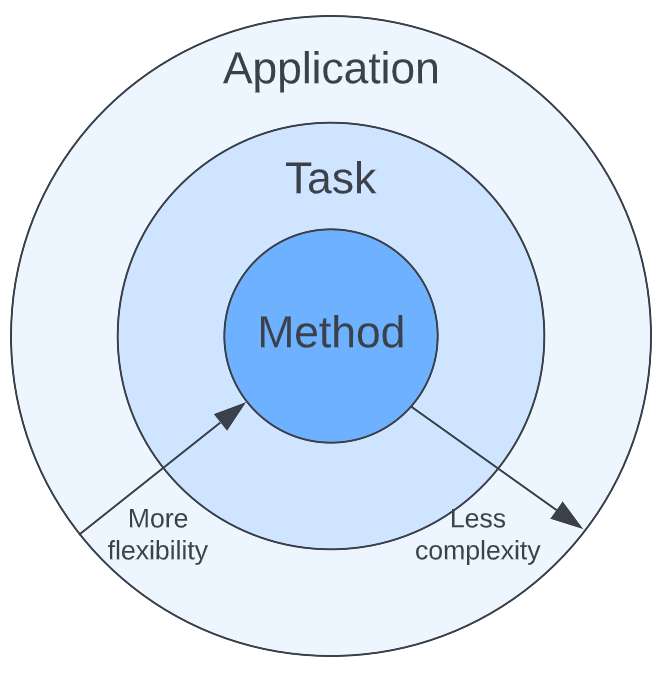
\includegraphics[width=0.4\textwidth]{figures/granularity.png}
	\caption{سه نوع دانه‌بندی مختلف در سامانه‌ی تخلیه‌ی پردازش}
	\label{fig:granularity}
\end{figure}

\subsection{تعداد کاربر و سرور}
در برخی از مقالات مانند \Cite{Liu} مسئله‌ی تخلیه‌ی پردازش تنها برای یک کاربر در نظر گرفته می‌شود، در حالیکه در برخی از مقالات مانند \Cite{multiuser} از چندین کاربر همزمان نیز پشتیبانی می‌شود. در \CurrentProject تعداد کاربران را برای سادگی یک در نظر می‌گیریم. طبیعتا در حالت تک‌کاربر نیز سرور خدمت‌دهنده می‌تواند به کاربران مختلفی خدمت‌دهی کند. اما تفاوتی که در این حالت وجود دارد این است که برای هر کاربر محیط تخلیه‌ی پردازش جدایی در نظر گرفته می‌شود و کاربران متفاوت از وضعیت یکدیگر اطلاعی ندارند. بنابراین در مقالاتی که تخلیه‌ی پردازش برای چندین کاربر در نظر گرفته می‌شود، عموما یک چاچوبی برای ارتباط و همکاری بین دستگاه‌های مختلف در شبکه نیز در نظر گرفته می‌شود. \\

مشابه با تعداد کاربران، تعداد سرورهای پردازشی در سامانه تخلیه نیز می‌تواند یک یا بیشتر باشد. برای نمونه در \Cite{multiuser} مسئله‌ی تخلیه‌ی پردازش برای چندین سرور بررسی شده است. در \CurrentProject ما حالت تک‌سرور را در نظر می‌گیریم. افزایش تعداد سرورها عموما فضای حالت مسئله بهینه‌سازی را بزرگ‌تر می‌کند، و حل آن را پیچیده‌تر.

\subsection{گره پردازشی}
در رایانش توزیع‌شده به انجام پردازش توسط هر گره پردازشی به جز گره ایجادکننده‌ی آن پردازش، تخلیه‌ی پردازش گفته می‌شود. با این حال بسته به نوع گره خدمت‌دهنده، مسئله تخلیه‌ی پردازش می‌تواند ویژگی‌های بسیار متفاوتی داشته باشد. در ادبیات تخلیه‌ی پردازش، عموما سه معماری مختلف برای سامانه در نظر گرفته می‌شود:
\begin{enumerate}
	\item پردازش در سرور ابری
	\item پردازش در سرور لبه‌ای
	\item پردازش در شبکه‌ای بدون ساختار (از دستگاه‌های کاربر)
\end{enumerate}
برای مثال در \Cite{Liu} گره‌های پردازشی سرورهای لبه‌ای در نظر گرفته شده است، در حالیکه در \Cite{kwak} مسئله‌ی تخلیه وظیفه در سطح رایانش ابری و به طور دقیق‌تر، «رایانش ابری متحرک\LTRfootnote{Mobile Cloud Computing}» بررسی شده است. در \Cite{manet} گره‌های پردازشی پهبادهای متحرک هستند و مسئله‌ی تخلیه وظیفه در محیط «شبکه بدون ساختار متحرک\LTRfootnote{Mobile Ad-hoc Network}» در نظر گرفته شده است. نوع گره‌های پردازشی همچنین بر روی «تحرک‌پذیری» دستگاه‌های کاربر تاثیر می‌گذارد. به طور کلی هر چه فاصله گره‌های پردازشی نسبت به دستگاه کاربر کمتر باشد و تعداد گره‌های پردازشی در حومه دستگاه کاربر بیشتر باشد، تحرک پذیری افزایش می‌یابد (مطابق شکل \ref{fig:mobility}).
\begin{figure}[H]
	\centering
	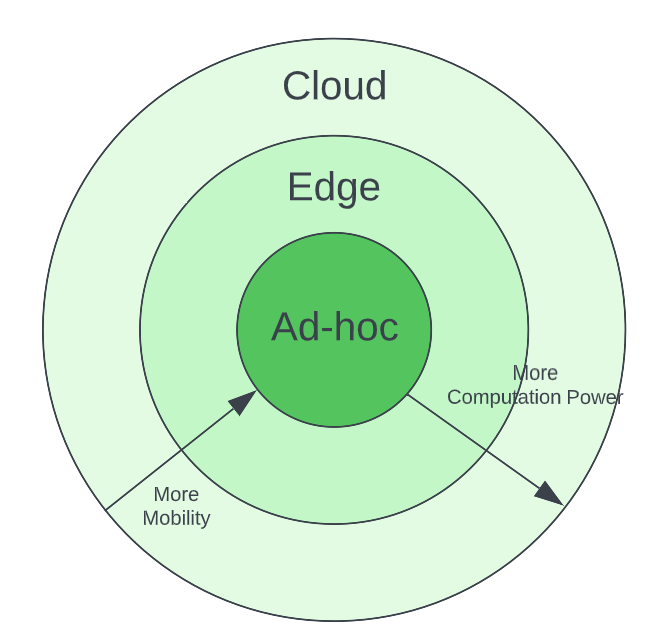
\includegraphics[width=0.4\textwidth]{figures/mobility.png}
	\caption{تحرک‌پذیری در سه نوع گره پردازشی مختلف}
	\label{fig:mobility}
\end{figure}

\subsection{معیار بهینه‌سازی}
 معیار بهینه‌سازی به کمیتی اشاره دارد که استراتژی تخلیه‌ی پردازش سعی در بهینه‌سازی آن دارد. برخی از معیارهای رایج عبارتند از: تاخیر، انرژی، کیفیت سرویس و هزینه. برای مثال در \Cite{Liu} معیار تاخیر، در \Cite{metricenergy} معیار انرژی و در \Cite{metriccost} معیار هزینه در نظر گرفته شده است.
\section{بررسی مقالات از نظر روش حل مسئله}
در جدول \ref{table:algorithms} که برگرفته از 
\Cite{Shakarami2020}
می‌باشد، یک دسته‌بندی کلی از الگوریتم‌های رایج برای حل مسئله‌ی تخلیه‌ی پردازش مشاهده می‌شود. در \CurrentProject ما از \textbf{روشی} قطعی بر پایه‌ی برنامه‌ریزی خطی برای یافتن \textbf{استراتژی تخلیه} تصادفی استفاده می‌کنیم. برای آشنایی بیشتر با روش‌های حل مسئله تخلیه وظیفه به\Cite{wang2019}
و \Cite{Shakarami2020} رجوع شود.

% Please add the following required packages to your document preamble:
% \usepackage{booktabs}
\begin{table}[H]
	\centering
	\begin{latin}
		\begin{tabular}{@{}ll@{}}
			\toprule
			\textbf{Model} & \textbf{Examples}                                                                                                                                                           \\ \midrule
			Stochastic     & \begin{tabular}[c]{@{}l@{}}Machine learning, \\ Generalized poison distribution, \\ Game theory, \\ Queuing theory, \\ Markov processes, \\ Gaussian processes\end{tabular} \\ \midrule
			Deterministic  & \begin{tabular}[c]{@{}l@{}}Some supervised Machine Learning approaches (e.g., KNN),\\ Linear and non-linear programming, \\ Linear regression equation\end{tabular}        
		\end{tabular}
	\end{latin}
	\caption{تقسیم‌بندی الگوریتم‌های حل مسئله‌ی تخلیه‌ی پردازش}
	\label{table:algorithms}
\end{table}

\section{پژوهش‌های مرتبط}
در \Cite{Liu} مسئله‌ی تخلیه‌ی وظیفه‌ی تاخیر-کمینه با استفاده از روشی مبتنی بر زنجیره‌ی مارکوف و برنامه‌ریزی خطی حل شده است. در این پژوهش محیط تک کاربر و تک سرور در نظر گرفته شده است. نویسندگان این مقاله نشان می‌دهند که روش ارائه‌شده در درازمدت عملکرد بهینه دارد. با این حال روش ارائه شده توسط این مقاله چندین کاستی دارد، از جمله عدم پشتیبانی از وظایف با نیازمندی‌های پردازشی متفاوت و عدم پشتیبانی از موازی‌سازی. \CurrentProject گسترشی بر این مقاله است. \\

در \Cite{samanta} مکانزیم تخلیه‌ی وظیفه‌ای با هزینه‌ی کمینه در محیط رایانش لبه‌ای متحرک ارائه‌شده است. محیط در نظر گرفته شده از نظر ثابت بودن طول بازه‌های زمانی و تفاوت وظایف و همچنین نحوه‌ی تعریف مسئله‌ی بهینه‌سازی، شبیه به \CurrentProject می‌باشد. اما از نظر معیار و تعداد سرور متفاوت می‌باشد. روش بهینه‌سازی استفاده شده در \CurrentProject روش «ضرایب لاگرانژ» می‌باشد که عملکرد سریعی دارد اما لزوما جواب بهینه سراسری را پیدا نمی‌کند و فقط جواب‌های بهینه محلی را پیدا می‌کند. \\

در \Cite{kwak} و \Cite{jiang} مشابه با \CurrentProject، ناهمگونی وظایف و تقابل تاخیر و انرژی در نظر گرفته شده است. با این تفاوت که در این دو مقاله از روش بهینه‌سازی لیاپانوف استفاده شده است. همچنین این دو مقاله مسئله‌ی تخلیه‌ی وظیفه را در محیط رایانش ابری در نظر گرفته‌اند و نه رایانش لبه‌ای. علاوه بر این هیچ یک از این دو مقاله چارچوبی نرم‌افزاری برای حل مسئله در محیط‌های خاص ارائه نداده‌اند. \\

در \Cite{zhang2013} مسئله‌ی تخلیه و زمان‌بندی ارسال و اجرا به صورت همزمان در نظر گرفته شده است و کانال بیسیم به صورت تصادفی مدل شده است و از این ابعاد به \CurrentProject شباهت دارد. بر خلاف پروژه فعلی معیار بهینه‌سازی در این پروژه انرژی مصرفی است. روش ارائه‌شده عملکرد خوبی دارد و به میزان قابل توجی در انرژی مصرفی صرفه‌جویی می‌کند. با این حال مدل در نظر گرفته شده کاستی‌هایی دارد. یک ایراد اصلی فرض وجود تنها یک کاربرد در سیستم است. به عبارت دیگر تاخیر ایجاد شده به واسطه انتظار کاربردها در صف در نظر گرفته نشده است.

\clearpage
